% vim: set textwidth=78 autoindent:

\subsection{Plugin MapServer Export}\label{sec:mapserver_export}

% when the revision of a section has been finalized, 
% comment out the following line:
%\updatedisclaimer

Si può usare QGIS per 'comporre' la propria mappa aggiungendo e arrangiando i layers, simbolizzandoli, personalizzando i colori, e infine creando un map file per Mapserver. Per usare il plugin MapServer Export bisogna aver istallato Python >= 2.4 nel proprio sistema e aver compilato QGIS con il supporto per esso. Tutti i pacchetti binari includonoil supporto Python.

Il plugin MapServer Export in QGIS \CURRENT è un plugin Python, il che significa che viene caricato automaticamente nel  \filename{Gestore dei Plugin} come plugin core 
(see Section~\ref{sec:core_plugins}).

\subsubsection{Creare il file Progetto}

Il Plugin MapServer Export opera su un progetto QGIS salvato e 
\textbf{non} sui contenuti correnti della finestra aperta e della sua legenda. Questo ha generato confusione per molta gente.  Come descritto più avanti, prima di cominciare ad utilizzare il Plugin MapServer Expor, è necessario predisporre i layers vettoriali e raster che si vuole usare in MapServer e salvare queste impostazionoi nel file progetto QGIS

\begin{figure}[ht]
\begin{center}
  \caption{predisporre i layers vettoriali e rasterin un file progetto QGIS \nixcaption}
  \label{fig:mapserver_export_qgs}\smallskip
  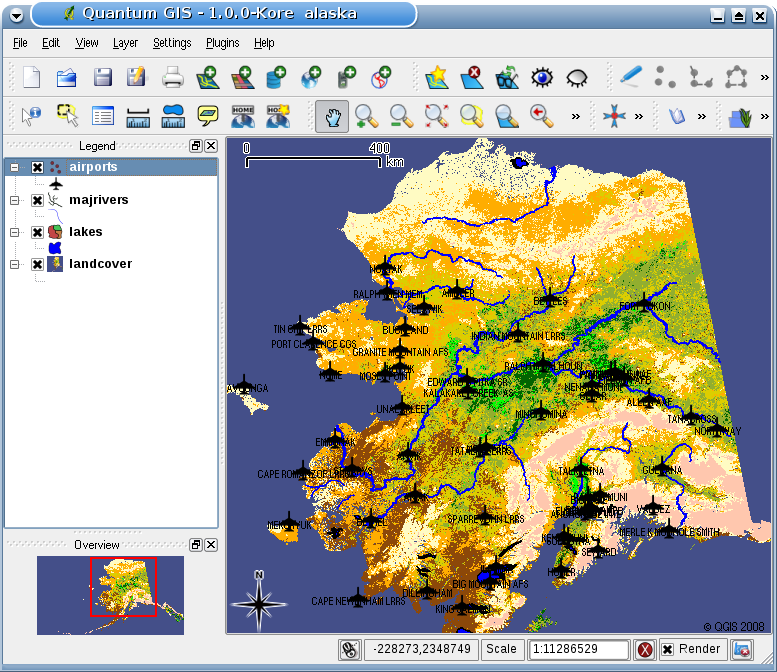
\includegraphics[clip=true, width=12cm]{mapserver_export_qgs}
\end{center}
\end{figure}

In questo esempio vengono mostrati i quattro passi per arrivare ad essere pronti a creare il map file in MapServer. Vengono usati file vettoriali e raster dal dataset campione di QGIS \ref{label_sampledata}.

\begin{enumerate}
\item Aggiungere il layer raster \filename{landcover.tif} premendo il tasto 
\toolbtntwo{mActionAddRasterLayer}{Aggiungere Layer Raster}.
\item Aggiungere i file Shape \filename{lakes.shp, majrivers.shp} e 
\filename{airports.shp} dal dataset campionei QGIS premendo il tasto 
\toolbtntwo{mActionAddNonDbLayer}{Aggiungere Layer Vettoriale} .
\item Cambiare i colri e simbilizzare i dati a piacere (vedere la Figura~\ref{fig:mapserver_export_qgs})
\item Salvare un nuovo progetto chiamato \filename{mapserverproject.qgs} usando 
\mainmenuopt{File} > \dropmenuopttwo{mActionFileSave}{Salva Progetto}.
\end{enumerate} 

\subsubsection{Creazione del Map File}

Lo strumento \filename{msexport} per esportare un file progetto QGIS in un file mappa MapServer è istallato nella directory binaria QGIS e può essere usato indipendentemente da QGIS. da QGIs bisogna prima caricare il Plugin MapServer Export con il Gestore dei Plugin. 
Selezionare \mainmenuopt{Plugins} > \dropmenuopt{Gestione Plugins...} per aprire il Gestore dei Plugin, 
scegliere il Plugin MapServer Export e premere \button{OK}. Ora avviare la finestra di dialogo 
\toolbtntwo{mapserver_export}{MapServer Export} (vedere 
Figura~\ref{fig:mapserver_export_dialog}) premendo il tasto nel menu strumenti.

\begin{figure}[ht]
\begin{center}
  \caption{Finestra di dialogo MapServer Export \nixcaption}
  \label{fig:mapserver_export_dialog}\smallskip
  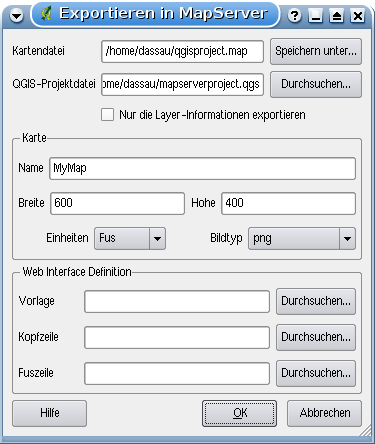
\includegraphics[clip=true, width=10cm]{mapserver_export_dialog}
\end{center}
\end{figure}

\begin{description}
\item [File mappa] \mbox{}\\
Scegliere un nome per il file mappa da creare. si può usare il tasto a destra per scegliere per la directory dove si vuole che il file venga creato. 
\item [File progetto QGIS] \mbox{}\\
Introdurre il percorso completo per il file progetto QGIS (.qgs) che si vuole esportare. Si può usare il tasto a destra per cercare il file progetto QGIS.
\item [Nome mappa] \mbox{}\\
Un nome per la mappa. Questo nome è prefissato a tutte le immagini generate dal mapserver.
\item [Larghezza mappa] \mbox{}\\
Larghezza dell'immagine in output in pixel.
\item [Altezza della mappa] \mbox{}\\
Altezza dell'immagine in output in pixel.
\item [Unità della mappa] \mbox{}\\
Unità di misura usate per l'output.
\item [Tipo di immagine] \mbox{}\\
Formato dell'immagine in output generata da MapServer.
\item [Modello web] \mbox{}\\
Percorso completo al file modello di Mapserver che sarà usato con il file mappa.
\item [Intestazione web] \mbox{}\\
Percorso completo al file intestazione di Mapserver che sarà usato con il file mappa.
\item [Piede pagina web] \mbox{}\\
Percorso completo al file piede pagina di Mapserver che sarà usato con il file mappa.
\end{description}

Soltanto gli input \filename{File Mappa} e \filename{file progetto QGIS} sono rchiesti per creare un file maoppa, tuttavia ci si può ritrovare con un file mappa non funzionante, a seconda di quale è l'uso che se ne vuole fare.Anche se QGIS è capace di creare un file mappa da un file progetto, può essere necessario qualche aggiustamento per raggiungere il risultato desiderato. Proviamo comunque a creare il file mappa usando il file progetto 
\filename{mapserverproject.qgs} appena creato 
(vedere Figura~\ref{fig:mapserver_export_dialog}):

\begin{enumerate}
  \item Aprire il Plugin MapServer Export premendo il tasto
  \toolbtntwo{mapserver_export}{MapServer Export}.
  \item Introdurre il nome \filename{qgisproject.map} per il nuovo file mappa.
  \item Selezionare il file progetto QGIS \filename{mapserverproject.qgs} appena salvato.
  \item Introdurre un nome \filename{mia_mappa} per la mappa.
  \item Introdurre \filename{600} per la larghezza e \filename{400} per l'altezza.
  \item I layer sono in metri, quindi si cambiano le unità a metri.
  \item Scegliere 'png' come tipo di immagine.
  \item Premere \button{OK} per generare il nuovo file mappa \filename{qgisproject.map}. 
  QGIS mostrerà il risultato.
\end{enumerate}

Si può visualizare il file mappa con qualsiasi editoreo visualizzatore  di testo. Se si apre il file, si noterà che lo strumeto di esportazione aggiunge i metadati necessari per abilitare la mappa per WMS. 

\subsubsection{Testare il Fle Mappa}

Si può testare il risultato fin qui ottenuto usando lo strumento \filename{shp2img} per creare un'immagine dal file mappa. L'utilità \filename{shp2img} è parte di MapServer e FWTools. 
Per creare un'immagine dalla mappa:

\begin{itemize}
\item Aprire una finestra terminale
\item Se la mappa on è stata salvata nella directory Home, cambiare alla cartelle in cui è stat salvata
\item Lanciare \filename{shp2img -m qgisproject.map -o mapserver\_test.png} e mostrare l'immagine 
\end{itemize}
 
Questo crea un PNG con tutti i layer inclusi nel file progetto QGIS. 
In aggiunta, l'estensione del PNG sarà la stessa di quando si è salvato il progetto.Come si vede in Figura~\ref{fig:mapserver_export_test}, tutte le informazioni eccetto i simboli degli aeroporti sono incluse.

\begin{figure}[ht]
\begin{center}
  \caption{Test PNG creato con shp2img con tutti i layer MapServer Export \nixcaption}
  \label{fig:mapserver_export_test}\smallskip
  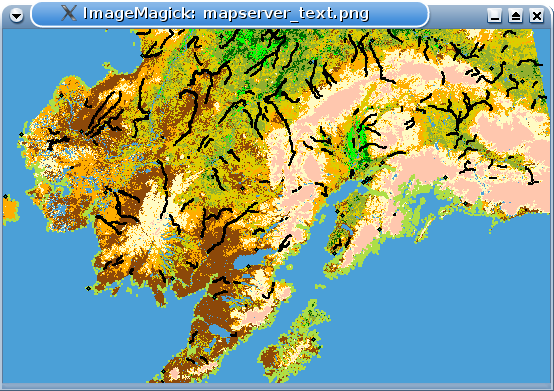
\includegraphics[clip=true, width=12cm]{mapserver_export_test}
\end{center}
\end{figure}

Se si prevede di usare il file mappa per rechieste WMS, probabilmente non sarà necessario alcun adattamento. Se invece si prevede di usarlo con un modello di mappatura o un'interfaccia personalizzata, potrebbe essere necessario un po' di lavoro. Per vedere come è facile passare da QGIS alle mappe di servizio sul web, vedere il flash video di 5 minuti di
Christopher Schmidt. Egli usa QGIS versione 0.8, ma è comunque utile.
\footnote{\url{http://openlayers.org/presentations/mappingyourdata/}}
